% Source: graduate-coursework/Research/Intro_to_Agents/slides/From_LLMs_to_Multi_Agent_Systems_slides.tex

\documentclass[border=4pt]{standalone}
\usepackage[T1]{fontenc}
\usepackage{graphicx}
\usepackage{tikz}
\usepackage{xcolor}
\usetikzlibrary{arrows.meta,positioning,shapes.geometric,fit,calc,
                decorations.pathreplacing,backgrounds,patterns,trees}

\definecolor{garnet}{HTML}{73000A}
\definecolor{rose}{HTML}{CC2E40}
\definecolor{atlantic}{HTML}{466A9F}
\definecolor{congaree}{HTML}{1F414D}
\definecolor{horseshoe}{HTML}{65780B}
\definecolor{grass}{HTML}{CED318}
\definecolor{honeycomb}{HTML}{A49137}
\definecolor{warmgrey}{HTML}{676156}
\definecolor{sandstorm}{HTML}{FFF2E3}
\definecolor{bk90}{HTML}{363636}
\definecolor{bk70}{HTML}{5C5C5C}
\definecolor{bk50}{HTML}{A2A2A2}
\definecolor{bk30}{HTML}{C7C7C7}
\definecolor{bk10}{HTML}{ECECEC}

\tikzset{
  agentbox/.style={
    rectangle, draw=#1, fill=#1!8, thick,
    minimum width=2.2cm, minimum height=0.8cm,
    font=\small\sffamily, align=center,
    inner sep=4pt
  },
  agentbox/.default=garnet,
  workerbox/.style={
    rectangle, draw=atlantic, fill=atlantic!8, thick,
    minimum width=1.8cm, minimum height=0.7cm,
    font=\small\sffamily, align=center,
    inner sep=3pt
  },
  tierbox/.style={
    rectangle, draw=#1, fill=#1!5, thick,
    minimum width=6.5cm, minimum height=1.0cm,
    font=\small\sffamily, align=center,
    inner sep=4pt
  },
  tierbox/.default=garnet,
  dataarrow/.style={
    -{Stealth[length=5pt]}, thick, color=#1
  },
  dataarrow/.default=bk70,
  brace/.style={
    decorate, decoration={brace, amplitude=6pt, raise=2pt}, thick, color=#1
  },
  brace/.default=bk50,
  labelnode/.style={
    font=\scriptsize\sffamily, color=bk70
  },
  codebox/.style={rectangle, draw=bk70, fill=bk90, text=white,
    font=\ttfamily\small, inner sep=6pt, align=left, text width=#1},
  codebox/.default=6cm,
  sysprompt/.style={rectangle, draw=rose, dashed, fill=rose!5, thick,
    minimum width=2.0cm, minimum height=0.6cm,
    font=\small\sffamily, align=center, inner sep=3pt},
  tooldef/.style={rectangle, draw=atlantic, fill=atlantic!8, thick,
    minimum width=1.8cm, minimum height=0.6cm,
    font=\small\sffamily, align=center, inner sep=3pt},
  wrapperbox/.style={rectangle, draw=garnet, dashed, thick, fill=garnet!3,
    inner sep=8pt},
  pbar/.style={rectangle, draw=#1, fill=#1!30, thick,
    minimum height=0.3cm, font=\scriptsize\sffamily},
  pbar/.default=horseshoe,
  flag/.style={rectangle, draw=rose, fill=rose!15, thick,
    minimum width=0.8cm, minimum height=0.4cm,
    font=\tiny\sffamily\bfseries},
  failbox/.style={rectangle, draw=rose, fill=rose!10, thick,
    font=\small\sffamily, align=center, inner sep=4pt},
}

\begin{document}
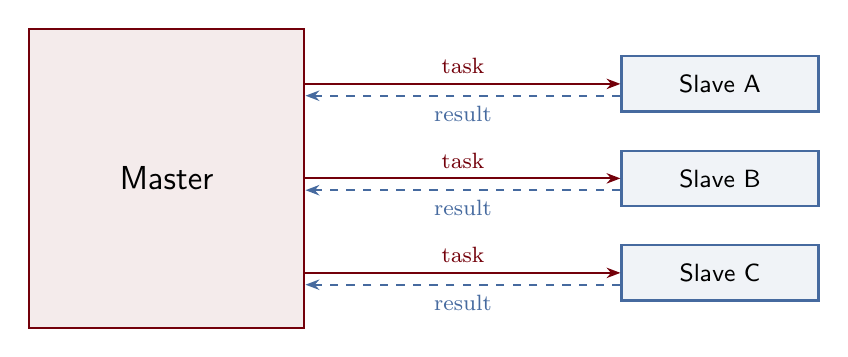
\begin{tikzpicture}[node distance=0.6cm]
\node[agentbox=garnet, minimum width=3.5cm, minimum height=3.8cm] (master) {\large Master};
\node[workerbox, right=4cm of master, yshift=1.2cm, minimum width=2.5cm] (w1) {Slave A};
\node[workerbox, right=4cm of master, yshift=0.0cm, minimum width=2.5cm] (w2) {Slave B};
\node[workerbox, right=4cm of master, yshift=-1.2cm, minimum width=2.5cm] (w3) {Slave C};
\draw[dataarrow=garnet] (master.east |- w1) -- (w1.west)
  node[midway, above, font=\footnotesize] {task};
\draw[dataarrow=garnet] (master.east |- w2) -- (w2.west)
  node[midway, above, font=\footnotesize] {task};
\draw[dataarrow=garnet] (master.east |- w3) -- (w3.west)
  node[midway, above, font=\footnotesize] {task};
\draw[dataarrow=atlantic, dashed] ([yshift=-0.15cm]w1.west) -- ([yshift=-0.15cm]master.east |- w1)
  node[midway, below, font=\footnotesize] {result};
\draw[dataarrow=atlantic, dashed] ([yshift=-0.15cm]w2.west) -- ([yshift=-0.15cm]master.east |- w2)
  node[midway, below, font=\footnotesize] {result};
\draw[dataarrow=atlantic, dashed] ([yshift=-0.15cm]w3.west) -- ([yshift=-0.15cm]master.east |- w3)
  node[midway, below, font=\footnotesize] {result};
\end{tikzpicture}
\end{document}
